\documentclass[11pt]{article}

\usepackage{amsmath}
\usepackage{amssymb}
\usepackage{amsthm}
\usepackage{hyperref}
\usepackage{graphicx}
\graphicspath{ {./img/} }

\setlength{\parindent}{0cm}
\let\emptyset\varnothing

\title{\textbf{MATH 2135 Linear Algebra} \\ 1.B Definition of Vector Space}
\author{Alyssa Motas}

\begin{document}

    \maketitle

    \pagebreak

    \tableofcontents

    \pagebreak

    \section{Definition}

    Let \textbf{F} be a field. A \emph{vector space} over \textbf{F} is a set $V$, together with a distinguished element \(0 \in V\) and with operations 
    \begin{align*}
        \text{addition} \qquad              & + : V \times V \rightarrow V \\
        \text{scalar multiplication} \qquad & \cdot : \textbf{F} \times V \rightarrow V.
    \end{align*}
    Satisfies the following 8 axioms:
    \begin{enumerate}
        \item[(A1)] Commutativity of addition. \[\forall v,w \in V, v + w = w + v\] 
        \item[(A2)] Associativity of addition. \[\forall v,w,u \in V, (v+w)+u = v+(w+u)\]
        \item[(A3)] Additive identity. \[\forall v \in V, 0 + v = v\]
        \item[(A4)] Additive inverse. \[\forall v \in V, \exists w \in V, v + w = 0\]
        \item[(M1)] Multiplicative identity. \[\forall v \in V, 1v = v\]
        \item[(M2)] Left distributivity. \[\forall a \in F, \forall v,w \in V, a(v+w) = av + aw\]
        \item[(M3)] Right distributivity. \[\forall a,b \in F, \forall v \in V, (a+b)v = av + bv\]
        \item[(M4)] Associativity of multiplication. \[\forall a,b \in F, \forall v \in V, (ab)v = a(bv)\]    
    \end{enumerate}

    \subsection{Terminology}

    \begin{itemize}
        \item The elements of \textbf{F} are called \emph{scalars}.
        \item The elements of $V$ are called \emph{vectors or points}.
        \item A vector space over \(\mathbb{R}\) is called a \emph{real vector space}.
        \item A vector space over \(\mathbb{C}\) is called a \emph{complex vector space}.
    \end{itemize}

    \pagebreak

    \section{Examples of Vector Spaces}

    \begin{enumerate}
        \item[(1)] \(\textbf{F}^n\) is the set of column vectors (sometimes row vectors) with elements from \textbf{F}. For instance, \(\mathbb{R}^n\) and \(\mathbb{C}^n\) are such vector spaces.
        \begin{align*}
            \textbf{F}^n &= \left\{ \begin{bmatrix}
                                        a_1    \\
                                        a_2    \\
                                        \vdots \\
                                        a_n
                                    \end{bmatrix} \mid a_1, \dots, a_n \in \textbf{F} \right\} \\
                         &= \{(a_1, a_2, \dots, a_n) \mid a_1, \dots, a_n \in \textbf{F}\}     \\
            0            = \begin{bmatrix}
                                0      \\
                                0      \\
                                \vdots \\
                                0
                            \end{bmatrix} \qquad
            \begin{bmatrix}
                a_1    \\
                \vdots \\
                a_n
            \end{bmatrix} &+ \begin{bmatrix}
                                b_1    \\
                                \vdots \\
                                b_n
                            \end{bmatrix} = \begin{bmatrix}
                                                a_1 + b_1 \\
                                                \vdots    \\
                                                a_n + b_n 
                                            \end{bmatrix} \qquad
            k \begin{bmatrix}
                a_1    \\
                \vdots \\
                a_n
              \end{bmatrix} = \begin{bmatrix}
                  k a_1  \\
                  \vdots \\
                  k a_n
              \end{bmatrix}
        \end{align*}
        The properties of \(\textbf{F}^n\) makes it a vector space. 

        \item[(2)] Let \(\textbf{F}^{\infty} = \{(x_1,x_2,x_3,x_4, \dots) \mid x_1,x_2,\dots \in \textbf{F}\}\) be the set of inifnite sequences of scalars. We define the following:
        \begin{itemize}
            \item \(0 = (0,0,0,\dots)\) is the constant zero sequences.
            \item If \(x = (x_1, x_2, x_3, \dots)\) and \(y = (y_1,y_2,y_3, \dots)\) then we define \[x + y = (x_1 + y_1, x_2 + y_2, \dots).\]
            \item If \(k \in \textbf{F}\) and \(x = (x_1,x_2,x_3, \dots)\), then we define \[kx = (kx_1, kx_2, \dots).\]
        \end{itemize}
        Then \(\textbf{F}^{\infty}\) is a vector space.  

        \pagebreak

        \item[(3)] Let \textbf{F} be a field and let $S$ be a set. Define \(\textbf{F}^{S} = \{f : S \rightarrow \textbf{F} \mid \text{$f$ is a function from $S$ to \textbf{F}}\}.\)
        
        \vspace{1em}

        Define \(0 \in \textbf{F}^{S}\) by \(0(x) = 0\). The $f$ is the zero function, $x$ is any element in $S$, which gives the output of 0. 

        \vspace{1em}

        If \(f,g \in \textbf{F}^{S}\), define \(f + g \in \textbf{F}^{S} \) as \[(f+g)(x) = f(x) + g(x).\]
        \begin{center}
            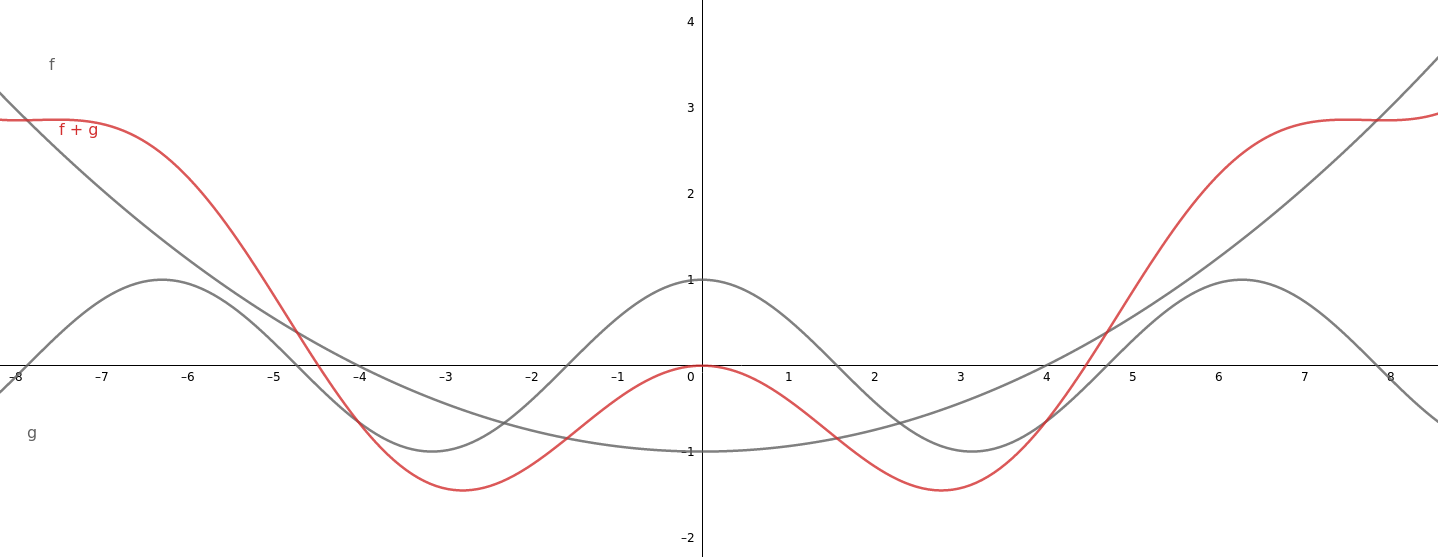
\includegraphics[width=\textwidth]{fg.png}
        \end{center}
        If \(k \in \textbf{F}\) and \(f \in \textbf{F}^{S}\), define \(kf \in \textbf{F}^{S}\) as \[(kf)(x) = k(f(x)).\]
        \begin{center}
            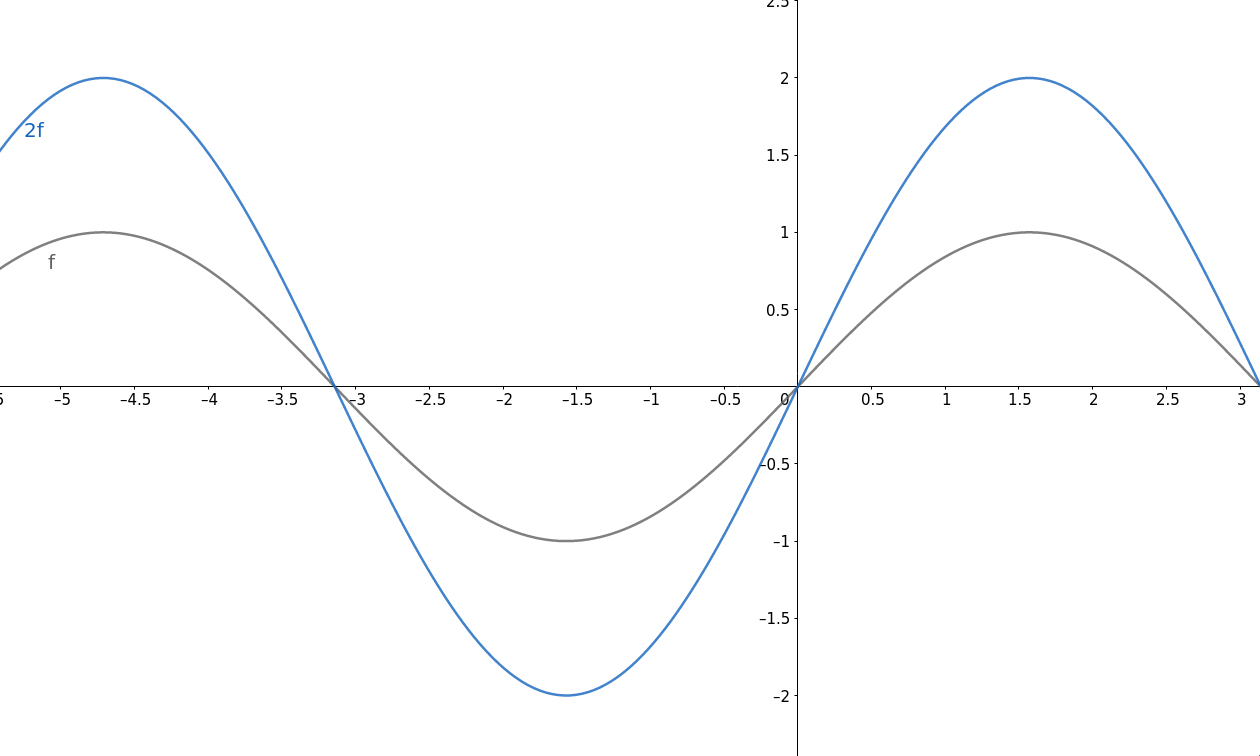
\includegraphics[width=10cm]{2f.png}
        \end{center}
        Then \(\textbf{F}^{S}\) is a vector space.

        \vspace{1em}

        \emph{Note:} The functions \(F,G : X \rightarrow Y\) are equal if \[\forall x \in X, F(x) = G(x).\]

        \begin{proof}
            Take arbitrary \(f,g \in \textbf{F}^{S}\). We have to show that \(f + g = g + f\) or \(\forall x \in S, (f + g)(x) = (g + f)(x).\) Suppose we take an arbitrary \(x \in S\), then we have
            \begin{align*}
                (f+g)(x) &= f(x) + g(x)                                       \\
                         &= g(x) + f(x) \quad \text{ by properties of fields} \\
                         &= (g+f)(x).
            \end{align*}  
            This finishes the proof of (A1). The other field axioms are similar.
        \end{proof}

        \item[(4)] For a field \textbf{F}, we define \(\mathcal{P}(\textbf{F})\) as the set of all formal polynomials with variable \(x\) and coefficients in \textbf{F}. \[\mathcal{P}(\textbf{F}) = \{a_0 + a_1 x + a_2 x^2 + \dots + a_n x^n \mid n \leq 0, a_0, \dots, a_n \in \textbf{F}\}.\] An example would be \(\mathcal{P}(x) = 3 + 5x - 7x^2.\)
        
        \vspace{1em}

        There are two ways to think about a polynomial: ``formal'' or ``function.'' For example, define the two following polynomials over \(\mathbb{Z}_2\) \[p(x) = x + 1 \qquad q(x) = x^2 + 1.\] As a function, it would be equal since:
        \begin{center}
            \begin{tabular}{| c | c | c |} \hline
                $x$ & $p(x)$ & $q(x)$ \\ \hline
                0   &   1    &   1    \\ \hline
                1   &   0    &   0    \\ \hline    
            \end{tabular}
        \end{center}
        As a formal polynomial, it would be different because it has the following form:
        \begin{align*}
            p(x) &= 0x^2 + 1x + 1 \\
            q(x) &= 1x^2 + 0x + 1.
        \end{align*}

        \pagebreak

        To prove that \(\mathcal{P}(\textbf{F})\) is a vector space, let us define the following:
        \begin{itemize}
            \item Zero polynomial. \[\mathcal{P}(x) = 0\]
            \item Addition.
            \begin{align*}
                p(x)        &= a_0 + a_1x + a_2 x^2 + \dots + a_n x^n \\
                q(x)        &= b_0 + b_1x + b_2 x^2 + \dots + b_n x^n \\
                \cline{1-2}
                (p + q)(x)  &= (a_0 + b_0) + (a_1 + b_1)x + (a_2 + b_2)x^2 + \dots + (a_n + b_n) x^n
            \end{align*}
            \item Scalar multiplication. \[kp(x) = (ka_0) + (ka_1)x + (ka_2) x^2 + \dots + (k a_n) x^n\]
        \end{itemize}
        With these operations, \(\mathcal{P}(\textbf{F})\) is a vector space.
    \end{enumerate}

    \pagebreak

    \section{Properties of Vector Spaces}

    Let $V$ be a vector space over a field \textbf{F}.
    \begin{itemize}
        \item The additive identity is unique. In other words, if \(u \in V\) is an additive identity (satisfying \(\forall v \in V, u + v = v\)) then \(u = 0\).
        \item Additive inverses are unique. Therefore, we can write \(-v\) for the additive inverse of \(v\). We also use related notations such as \(v-w\) to mean \(v + (-w)\).
        \item Cancellation of addition. \[v + w = u + w \Rightarrow v = u\]
        \item For all \(v \in V\), we have \[0v = 0.\] The 0 is a scalar being multiplied by $v$ (vector), and the 0 on the right is the zero vector.
        \begin{proof}
            We have
            \begin{align*}
                0v + 0v &= (0 + 0)v && \text{by (M3)}                  \\
                        &= 0v       && \text{by properties of scalars} \\
                        &= 0 + 0v   && \text{by (A3)}
            \end{align*}
            So \(0v = 0\) follows by cancellation.
        \end{proof}
        \item For all scalars \(a \in \textbf{F}\), we have \[a0 = 0.\]
        \begin{proof}
            We have
            \begin{align*}
                a0 + a0 &= a(0 + 0) && \text{by (M2)} \\
                        &= a0       && \text{by (A3)} \\
                        &= 0 + a0   && \text{by (A3)}
            \end{align*}
            So \(a0 = 0\) follows by cancellation.
        \end{proof}
        \item For all \(v \in V\), we have \[(-1)v = -v.\]
        \begin{proof}
            We have
            \begin{align*}
                (-v) + v &= v + (-v) && \text{by (A1)} \\
                         &= 0.       && \text{by (A4)}
            \end{align*}
            We also have
            \begin{align*}
                (-1)v + v &= (-1)v + 1v && \text{by (M1)} \\
                          &= (-1 + 1)v  && \text{by (M3)} \\
                          &= 0v         && \text{by properties of scalars} \\
                          &= 0.         && \text{by a previously proved property}
            \end{align*}
            In particular, \[(-v) + v = (-1)v + v.\] Then the claim \(-v = (-1)v\) follows by cancellation.
        \end{proof}
    \end{itemize}

    \end{document}